\documentclass[11pt]{article}
\usepackage{acl2016}
\usepackage{url}
%\usepackage{latexsym}
\usepackage[T1]{fontenc}
\usepackage{times}
\usepackage[utf8]{inputenc}
\usepackage[english]{babel}
\usepackage{natbib}
\usepackage{hyperref}
\usepackage{amsmath,amssymb,amsfonts,amsthm,amstext,amscd}
%\usepackage[usenames, dvipsnames]{color}

%\newcommand{\huang}{\texttt{huang}}
\newcommand{\neelakantan}{\texttt{neela}}
\newcommand{\adagram}{\texttt{AdaGram}}
\newcommand{\mutli}{\texttt{mutli}}
\newcommand{\Ro}{\mathbb{R}^{d_1}}
\newcommand{\Rt}{\mathbb{R}^{d_2}}
\newcommand{\fl}{\texttt{4lang}}
\newcommand{\any}{\texttt{any}}
\newcommand{\disamb}{\texttt{disamb}}

\usepackage{tikz}
\definecolor{hltblue}{RGB}{3,61,92}
\definecolor{hltdarkgreen}{RGB}{26,148,129}
\definecolor{hltlightgreen}{RGB}{155,204,147}
\definecolor{hltyellow}{RGB}{252,238,166}

\usepackage{booktabs}
\usepackage{multirow}%,multicol}
\usepackage{cleveref}
%\usepackage{graphicx}
%\usepackage{dblfloatfix}
%\usepackage{array}
%\usepackage{changepage}

\hyphenation{poly-semy}\hyphenation{Web-kor-pusz}
%\usepackage{dcolumn}
%\newcolumntype{d}[1]{D{.}{.}{#1}}

\usepackage{todonotes}
%\newcommand{\todo}[1]{}
\usepackage{wasysym}

\newcommand{\paprika}{
\begin{figure}
\includegraphics[width=.9\columnwidth]{paprika}
\end{figure}
}

\aclfinalcopy % Uncomment this line for the final submission
%\def\aclpaperid{28} %  Enter the acl Paper ID here

%\setlength\titlebox{8cm}
%\setlength\titlebox{50ex}  % Vertical space allocated for \Authors
% You can expand the titlebox if you need extra space
% to show all the authors. Please do not make the titlebox
% smaller than 5cm (the original size); we will check this
% in the camera-ready version and ask you to change it back.

\title{Do multi-sense embeddings learn more senses? \\ An evalutaion in linear
translation}
\author{
  Márton Makrai
  \\ Institute for Linguistics\\
  Hungarian Academy of Sciences \\
  %Bencz\'ur u. 33 \\ 1068 Budapest, Hungary \\
  \href{mailto:makrai.hlt@gmail.com}{makrai.marton@nytud.mta.hu} \\
}
\date{}


\begin{document}
\maketitle

%\hspace{2cm}

%\begin{abstract}
%As far as we now, we are the fist to test the effect of orthogonality
%constraint and related vector preprocessing techniques in reverse nearest
%neighbour seach.
%\end{abstract}


\emph{Word sense induction} (WSI) is the task of discovering senses of words
without supervision \citep{Schutze:1998}. Recent approaches include multi-sense
word embeddings (MSEs), vector space models of word distribution with more
vectors for ambiguous words. In MSEs, each vector is supposed to corresponding
to a different word sense, but in practice vectors seem to duplicate senses.

In \cite{Borbely:2016}, we proposed a cross-lingual method for the evaluation
of the sense resolution in MSEs. The method is based on the principle that
words may be ambiguous as far as the postulated senses translate to different
words in some other language.  For the translation of words, we applied the
method by \citet{Mikolov:2013x} who train a translation mapping from the source
languages embedding to the target as a least-squares regression supervised by a
seed dictionary of the few thousand most frequent words. The translation of a
source word vector is the nearest neighbor of its image by the mapping in the
target space. In the multi-sense setting, we have translated from MSEs. (The
target embedding remained single-sense.)

Now we develop the evaluation further. Part of the evaluation task is to decide
on empirical grounds whether different good translations of a word are synonyms
or translations in different senses.  The reader should be noted that the
evaluation is not very strict, rather a process of discovering something
meaningful in present-day MSE implementations.\footnote{The code for these
experiments can be found at \url{https://github.com/makrai/wsi-fest}.}

\section{Towards a less \emph{delicious} inventory}

\begin{figure}
    \centering
    \resizebox{\columnwidth}{!} {
        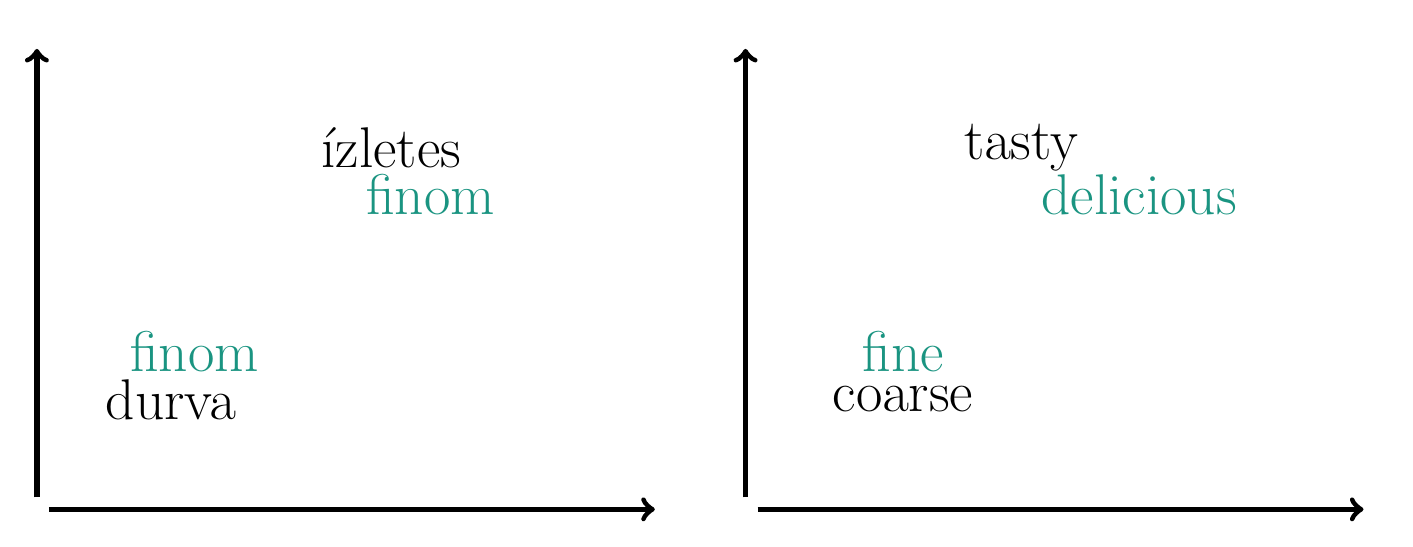
\begin{tikzpicture}[line width=2pt] %[&gt;=stealth']
            \tikzstyle{every node}=[font=\huge]
            %\tikzset{every edge thick}
            \node[text=hltdarkgreen] (hf) at (2, 2) {finom};
            \node (hf) at (1.7, 1.4)  {durva};
            \node[text=hltdarkgreen] (hs) at (5, 4)  {finom};
            \node (hs) at (4.5, 4.6)  {ízletes};
            \node[text=hltdarkgreen] (gf) at (11, 2) {fine};
            \node (gf) at (11, 1.4) {coarse};
            \node[text=hltdarkgreen] (gs) at (14, 4) {delicious};
            \node (gs) at (12.5, 4.6) {tasty};
            \node (ho) at (0, 0) {};
            \node (hx) at (8, 0) {};
            \node (hy) at (0, 6) {};
            \node (go) at (9,0) {};
            \node (gx) at (17,0) {};
            \node (gy) at (9,6) {};

            \draw[->] (ho) edge (hx);
            \draw[->] (ho) edge (hy);
            \draw[->] (go) edge (gx);
            \draw[->] (go) edge (gy);
        \end{tikzpicture}
    }
    \caption{Linear translation of word senses. The Hungarian word
        \emph{finom} is ambiguous between `fine' and `delicious'.}
        \label{fig:AdaGram}
\end{figure}


We emphasize that our evaluation proposal probes an aspect of MSEs,
\emph{semantic resolution}, which is not well measured by the well-known word
sense disambiguation (WSD) task that aims at classifying occurrences of a word
form to different elements of a sense inventory pre-defined by some experts.
Our goal in WSI is to probe the granularity of the inventory itself.  The
differentiation of word senses, as already noted in \cite{Borbely:2016}, is
fraught with difficulties, especially when we wish to distinguish homophony,
using the same written or spoken form to express different concepts, such as
Russian {\it mir} `world' and {\it mir} `peace' from polysemy, where speakers
feel that the two senses are very strongly connected, such as in Hungarian {\it
nap} `day' and {\it nap} `sun'.

% To quote \cite{Zgusta:1971} ``Of course it is a pity that we have to rely on
% the subjective interpretations of the speakers, but we have hardly anything
% else on hand''.
% Etymology
% Different languages make different lump/split decisions in the conceptual
% space, so much so that translational relatedness can, to a remarkable extent,
% be used to recover the universal clustering \citep{Youn:2016}.

The goal of WSI can be set at two levels. We may more modestly aim to
distinguish homophony from polysemy. In ideal case, we could even differentiate
between metonymy and metaphor, two subtypes of polysemy, that are discussed in
the next section, by Veronika Lipp, in more detail.  

\subsection{Lexicographic Background \\ (Veronika Lipp)}

\label{sec:bground}

Lexical ambiguity is linguistically subdivided into two main categories:
\emph{homonymy and polysemy} \citep{Cruse:2004}. Homonymous words have
semantically unrelated and mutually incompatible meanings, such as
\emph{punch$_1$} , which means `a blow with a fist', and \emph{punch$_2$},
which means `a drink'. Some have described such homonymous word meanings as
essentially distinct words that accidentally have the same phonology (e.g.,
Murphy, 2002). Polysemous words, on the other hand, have semantically related
or overlapping senses (\cite{Cruse:2004,Jackendoff:2002, Pustejovsky:1995}),
such as \emph{mouth} meaning both `organ of body' and `entrance of cave'.

Two criteria have been proposed for the distinction between homonymy and
polysemy. The first criterion has to do with the \emph{etymological} derivation
of words. Words that are historically derived from distinct lexical items are
taken to be homonymous. However, the etymological criterion is not always
decisive. One reason is that there are many words whose historical derivation
is uncertain. Another reason is that it is not always very clear how far back
we should go in tracing the history of words \citep{Lyons:1977}.

The second criterion for the distinction between homonymy and polysemy has to
do with the \emph{relatedness/unrelatedness of meaning}.  The distinction
between homonymy and polysemy seems to correlate with the native speaker’s
feeling that certain meanings are connected and that others are not. Generally,
unrelatedness in meaning points to homonymy, whereas relatedness in meaning
points to polysemy.  However, in a large number of cases, there does not seem
to be an agreement among native speakers as to whether the meanings of the
words are related. So, it seems that there is not a clear dichotomy between
homonymy and polysemy, but rather a continuum from ‘‘pure’’ homonymy to
‘‘pure’’ polysemy \citep{Lyons:1977}.

Most discussions about lexical ambiguity, within theoretical and computational
linguistics, concentrate on polysemy, which can be further divided into two
types (c.f. \cite{Apresjan:1974,Pustejovsky:1995}). The first type of polysemy
is motivated by \emph{metaphor (irregular polysemy)}. In metaphorical polysemy,
a relation of analogy is assumed to hold between the senses of the word. The
basic sense of metaphorical polysemy is literal, whereas its secondary sense is
figurative. For example, the ambiguous word \emph{eye} has the literal basic
sense  `organ of the body' and the figurative secondary sense `hole in a
needle.' The other type of polysemy is motivated by \emph{metonymy (regular
polysemy)}. In metonymy, the relation that is assumed to hold between the
senses of the word is that of contiguity or connectedness.
% Apresjan argued that metonymically motivated polysemy respects the usual
% notion of polysemy, which is the ability of a word to have several distinct
% but related meanings.
In metonymic polysemy, both the basic and the secondary senses are literal. For
example, the ambiguous word \emph{chicken} has the literal basic sense
referring to the animal and the literal secondary sense of the meat of that
animal.

% ``After centuries of practical lexicography, there is still hardly any
% consensus on how to divide the semantic space of a lexical item''
% \citep{Meer:2006}, how many senses a word has, and in which order they should
% be presented.  Senses of polysemous words can be described at different levels
% of granularity, either more towards broader categories (lumping) or
% fine-grained ones (splitting), depending on the purpose of the dictionary, its
% size, target users etc.  Dictionaries, even those for the same types of users
% and of similar size, offer (very) different sense division of many words.
%
% While homonyms with their non-overlapping semantic fields easily lend
% themselves to \emph{sense-tagging}, polysemic meanings pose real challenge.
% Lexicons may comprise overlapping meanings, which render the unique assignment
% of the right meaning to the given word impossible even for human annotators.

% Collocations, semantic associations and colligations of a word play a
% decisive role in differentiating between its senses (lexical priming,
% \cite{Hoey:2005}).

\section{Multi-sense word embeddings}

Vector-space language models with more vectors for each meaning of a
word originate with \cite{Reisinger:2010}.
\cite{Huang:2012} trained the first neural-network-based MSE.
Both works use a uniform number of clusters for all words that they select
before training as potentially ambiguous.
The first system with adaptive sense numbers and an effective open-source
implementation is the
modification of skip-gram \cite{Mikolov:2013d}, multi-sense skip-gram by
\cite{Neelakantan:2014}, where new senses are introduced during training by
thresholding the similarity of the present context to earlier contexts.

% \cite{Tian:2014}, Guo et al., 2014, Wu and Giles, 2015, Liu et al., 2015, Vu
% and Parker 2016, Šuster et al., 2016

% \citep{Neelakantan:2015, Bartunov:2015} improve upon the predecessors in
% three aspects: they do word sense discrimination simultaneously with the
% training of word embeddings, they determine the number of meanings based on
% the similarities of exemplars to global vectors, and make the system
% computationally more efficient.

\cite{Bartunov:2015} and \cite{Li:2015} improve upon the heuristic thresholding
by formulating text generation as a Dirichlet process. In
\adagram~\citep{Bartunov:2015}, senses may be merged as well as allocated
during training. \mutli-sense skip-gram\footnote{Note the $l\leftrightarrow
t$ metathesis in the name of the repo which is the only way of distinguishing it
from the other two multi-sense skip-gram models.} \citep{Li:2015} applies the
Chinese restaurant process formalization of the Dirichlet process. Both
\adagram~and \mutli~have a parameter for semantics resolution (more or less
senses) $\alpha$ and $\gamma$ respectively.

% https://sites.google.com/site/senseworkshop2017/

% Sense representations have been already used for several NLP tasks
% such as text classification (Li and Jurafsky, 2015, Flekova and Gurevych,
% 2016) and knowledge base construction (Delli Bovi et al. 2015, Espinosa-Anke
% et al. 2016) and completion (Bordes et al. 2013, Wang et al. 2014)},
MSEs are yet in research phase: \cite{Li:2015}  demonstrate that, when
meta-parameters are carefully controlled for, MSEs introduce a slight
performance boost in semantics-related tasks (semantic similarity for words and
sentences, semantic relation identification, part-of-speech tagging), but
similar improvements can also e achieved by simply increasing the dimension of
a single-sense embedding.

\section{Linear translation from MSEs}

 \cite{Mikolov:2013x} discovered that embeddings of different languages are so
 similar that a linear transformation can map vectors of the source language
 words to the vectors of their translations.

The method uses a seed dictionary of a few thousand words to learn translation
as a linear mapping $W: \mathbb{R}^{d_1}\rightarrow \mathbb{R}^{d_2}$ from the
source (monolingual) embedding to the target: the translation $z_i \in \Rt$ of
a source word $x_i \in \Ro$ is approximately its image $Wx_i$ by the mapping.
The translation model is trained with linear regression on the seed dictionary

\[\min_W \sum_i || Wx_i - z_i ||^2 \]
and can be used to collect translations for the whole vocabulary by choosing
$z_i$ to be the nearest neighbor (NN) of $Wx_i$.  We follow
\cite{Mikolov:2013x} in using different metrics, Euclidean distance in training
and cosine similarity in collection of translations.

In a multi-sense embedding scenario, \cite{Borbely:2016} take an MSE as the
source model, and a single-sense embedding as target.  The quality of the
translation has been measured by training on the most frequent 5k word pairs
and evaluating on another 1k seed pairs.

\subsection{Reverse nearest neighbor search}

% First, worse method by Dinu:2015: they sample additional vectors in the
% source domain called \emph{pivots} besides the test words, and normalize the
% vector of similarities of each target item to the mapped pivots to length 1.

A common problem when looking for nearest neighbors in high-dimensional spaces
\citep{Radovanovic:2010,Suzuki:2013,Tomasev:2013}, and especially in
embedding-based dictionary induction \citep{Dinu:2015,Lazaridou:2015} is when
there are \emph{hubs}, data points (target words) returned as the NN
(translation) of many points ($Wx$s), which is wrong (translation) in most of
the cases.  \cite{Dinu:2015} attack the problem explicitly with a method they
call \emph{global correction}.  Here, instead of the original NN that we will
call \emph{forward} NN search to contrast with the more sophisticated method,
they first rank source words by their similarity to target words. In
\emph{reverse} nearest neighbor (rNN) search, source words are translated to
the target words to which they have the lowest (forward) NN rank.\footnote{If
more target words have the same forward rank, \cite{Dinu:2015} make the
decision based on cosine similarity. This tie braking has not proven useful in
our experiments.}

We found that in reverse NN search it is important to restrict the vocabulary to
the some tens of thousands most frequent words not only for memory saving (the
$|V_{sr}|\times|V_{tg}|$ similarity matrix has to be sorted column-wise for
forward and row-wise for reverse ranking, so at some point of the computation
we keep the whole integer matrix of forward NN ranks in memory), a vocabulary
cutoff of $2^{15}=32768$ both on the source and the target size yields slightly
better results (74.3\%) than the more ambitious $2^{16}=65536$ (73.9\%). This
is not the case for forward NN search, where accuracy increases with vocabulary
limit (but remains far below that of reverse NN).

\subsection{Orthogonal restriction and other tricks}

\newcommand{\wordtovec}{\texttt{word2vec}}

\cite{Xing:2015} notes that the original linear translation method is
theoretically inconsistent being based on three different similarity measures:
\wordtovec~itself uses the dot-product of unnormalized vectors, the translation
is trained based on Euclidean distance, and neighbors are queried based on
cosine similarity. They make the framework more coherent by length-normalizing
the embeddings, and restricting $W$ to preserve vector length: their matrix
$W$ is orthogonal, i.e.~the mapping is a rotation.  \citep{Faruqui:2014} gains
even better results by mapping the two embeddings to a lower-dimensional
bilingual space with canonical correlation analysis.  \citep{Artetxe:2016}
analyses elements of these two works both theoretically and empirically, and
find a combination that improves upon dictionary generation and also preserves
analogies \citep{Mikolov:2013l} like

\[\mathbf{woman} + \mathbf{king}- \mathbf{man}  \approx \mathbf{queen}\]
among the mapped points $Wx_i$. They find that the
orthogonality constraint is key to preserve performance in analogies, and it
also improves bilingual performance.  In their experiments, length
normalization, when followed by centering the embeddings to $\mathbf 0$ mean,
obtains further improvements in bilingual performance without hurting
monolingual performance.

We also implemented the orthogonal restriction by computing the singular value
decomposition

\[U\Sigma V=S_t^\top T_t\] where $S_t$ and $T_t$ are the matrices consisting of
the embedding vectors of
the training words pairs in the source and the target space respectively, and
taking

\[W=U\mathbf{1}V\]
where $\mathbf 1$ is the rectangular identity matrix of appropriate shape.

\begin{table*}
  \resizebox{\textwidth}{!}{%
  \begin{tabular}{ll|llll|llll|llll}
    \toprule
    && \multicolumn{4}{c|}{8192} & \multicolumn{4}{c|}{16384} & \multicolumn{4}{c}{32768} \\
    && \multicolumn{2}{c}{general linear} & \multicolumn{2}{c|}{orthogonal} &
    \multicolumn{2}{c}{general linear} & \multicolumn{2}{c|}{orthogonal} &
    \multicolumn{2}{c}{general linear} & \multicolumn{2}{c}{orthogonal} \\
    && any & disamb & any & disamb & any & disamb & any & disamb & any & disamb & any & disamb \\
    \midrule
    \multirow{3}{*}{\rotatebox[origin=c]{90}{fwd}}
    & vanilla & 28.7\%	&  2.40\%	&  32.1\%	&  2.40\%	&  36.2\%	&  3.40\%	&  42.0\%	&
    4.70\%	& 36.7\%	&  4.20\%	&  44.5\%	&  6.00\%	\\
    & normalize & 28.2\%	&  2.20\%	& {\bf 33.7\%}	& 3.40\%	&  35.1\%	&
    2.80\%	&  {\bf 44.4\%}	&
    5.80\%	&  36.6\%	& 3.80\%	& {\bf 48.2\%}	&  6.00\%	\\
    & + center &  26.6\%	&  2.10\%	& 32.8\%	&  2.90\%	& 32.9\%	& 2.70\%	&  42.0\%	&
    4.50\%	&  34.6\%	& 3.50\%	&  43.9\%	& 5.50\%	\\
    \midrule
    \multirow{3}{*}{\rotatebox[origin=c]{90}{rev}}
    & vanilla & {\bf 53.8\%}	&  11.85\%	& 51.7\%	&  11.37\%	& {\bf 58.3\%}	&  11.99\%	& 56.6\% &
    12.59\%	&  {\bf 74.3\%}	& 23.60\%	&  73.6\%	& 22.30\%	\\
    & normalize &  53.3\%	& 11.61\%	 & 50.0\%	&  10.90\%	& 58.0\%	&  12.35\%	& 56.5\% &
    12.59\%	& 73.7\%	& 24.20\%	&  72.8\%	& 22.10\%	\\
    & + center &  51.7\%	& 11.37\%	& 53.3\%	& 11.14\%	&  57.1\%	&  11.99\%	& 57.7\% &
    12.35\%	& 69.7\%	& 22.20\%	& 73.5\%	&  23.00\%	\\
    \bottomrule
  \end{tabular}
  }
  \caption{Precision@10 of forward and reverse NN translations with and
  without the orthogonality constraint and related techniques at vocabulary
  cutoffs 8192 to 32768. (\any~and \disamb~will be explained in
  \cref{sec:res}.) The source has been an \adagram~model in 800 dimensions,
  $\alpha=.1$, trained on Webkorpusz with the vocabulary cut off at 8192 sense
  vectors.}
  \label{tab:orthog}
\end{table*}

\Cref{tab:orthog} shows our experimental results. Precision in forward NN
search is similar to that in Xing et al.~(\citeyear{Xing:2015}) and
\cite{Artetxe:2016}: the best combination is an orthogonal mapping between
length-normalized vectors, however, centering did not help in our experiments.
Reverse NNs are quite different: none of the orthogonality-related techniques
help. 

\section{Experiments}

\subsection{Data}

We trained \neelakantan, \adagram~and \mutli~models on (original and stemmed
forms of) two semi-gigaword (.7--.8 B words) Hungarian corpora, the Hungarian
Wecorpus (Webkorpusz, \cite{Halacsy:2004}) and (the non-social-media part of)
the Hungarian National Corpus (HNC, \cite{Oravecz:2014}).  We used Wiktionary
as our seed dictionary, extracted with
\texttt{wikt2dict}\footnote{\url{https://github.com/juditacs/wikt2dict}}
\citep{Acs:2013}. We tried several English embeddings as target, including the
300 dimensional skip-gram with negative sampling model \texttt{GoogleNews}
released with
\wordtovec~\citep{Mikolov:2013f}\footnote{\url{https://code.google.com/archive/p/word2vec/}},
and those released with GloVe
\citep{Pennington:2014}\footnote{\url{https://nlp.stanford.edu/projects/glove/}}.

\subsection{Results}

\label{sec:res}


We evaluate MSE models in two ways referred to as \any~and \disamb.  The method
\any~has been used for tuning the (meta)parameters of the source embedding and
to choose the target: a traditional, single-sense translation has been trained
between the first \todo{all} sense vector of each word form and its
translations. (If the training word is ambiguous in the seed dictionary, all
translations have been included in the training data.)  Exploiting the multiple
sense vectors, one word can have more than one translation.  During test, a
source word was accepted if \any~\todo{the 1st}of its sense vectors had at
least one good translation among its $k$ reverse nearest neighbors (rNN@$k$).
\Cref{tab:prec} shows results by the best models.

\begin{table}
  \centering\small
  %\resizebox{\columnwidth}{!}{%
    \begin{tabular}{lcccc|cc}
      \toprule
        & dim & $\alpha/\gamma$ & $p$ & $m$ & any & disamb \\
        % & \multicolumn{6}{c|}{forward NN search} & \multicolumn{6}{c}{reverse NN search} \\
      %vocab cutoff &&&&& \multicolumn{2}{c}{8192} & \multicolumn{2}{c}{16384} & \multicolumn{2}{c|}{32768} & \multicolumn{2}{c}{8192} & \multicolumn{2}{c}{16384} & \multicolumn{2}{c}{32768} \\
      \midrule
      %/jiweil/mnsz/stemmed/mnsz-stemmed-CRP-800-w15-joint_vect_sense.mse 23.0% 2.200%
      %/jiweil/mnsz/stemmed/mnsz-stemmed-CRP-800-w15-joint_vect_sense_context.mse 26.1% 3.300%
      %/neelakantan/mnsz/stemmed/mnsz2-stemmed-neela-np-800-s2_cluscent.mse 36.3% 6.400%
      %/neelakantan/webkorp_1-sense_sense.mse 37.8% 5.900%
      %/neelakantan/mnsz/stemmed/mnsz2-stemmed-neela-np-800-s2_sense.mse 38.1% 6.500%
      HNC	        & 800	& .02	&       & 100   & 48.5\%	&  7.6\% \\
      \neelakantan~Wk&300&--&2   &big  & 54.0\%	&  12.4\% \\
      HNC stem & 800	& .05	&       &  big & 55.1\%	&  10.4\% \\
      %	& \mutli~Webkorp\footnotemark  &&&&    & 1.0 & 55.0% 13.5\% \\
      HNC         & 160 & .05 & 3     & 200   & 62.2\%	&  15.0\% \\
      \mutli~Wk &300&.25 &       & 71    & 62.9\%	&  17.4\% \\
      Webkorpusz	    & 800	& .05	&       & 100	  & 65.9\%	&  17.4\% \\
      HNC	        & 600	& .05	& 5     & 100	  & 68.6\%	&  16.6\% \\
      HNC	        & 600	& .1  & 3     & 50	  & 69.1\%	&  18.8\% \\
      Webkorpusz	    & 800	& .1  &       & 100	  & 73.9\%	&  23.9\% \\
      \bottomrule 
    \end{tabular}
  %}
  \caption{Precision of \any~reverse NN and the number of word forms with
  non-synonymic vectors (\disamb).  The source embedding has been trained with
  \adagram, except for when indicated otherwise (\neelakantan, \mutli).  The
  meta-parameters are $d$imension, the resolution parameter ($\alpha$ in
  \adagram and $\gamma$ in \mutli), the maximum number of $p$rototypes (sense
  vectors), and the vocabulary cutoff ($m$in-freq). The two models with
  \emph{big} have technically no cut-off.}
    \label{tab:prec}
\end{table}

In \disamb, we used the same translation matrix as in \any, and inspected the
translations of the different sense vectors to see whether the vectors really
model different senses rather than synonyms.
% We separated \emph{common} translations of word vectors, i.e.~translations
% $t$ of a source word such that all the source sense vectors that have at
% least one good translation have $t$ among their translations.  Common
% translations do not evidence different senses. Instead
The lowest requirement for sense vectors $s_1, s_2$ for not being synonyms is
that the sets of corresponding good rNN@$k$ translations are different. The
ratio of words satisfying this requirement among all words with more than one
sense vector is show as \disamb~in \cref{tab:prec}. The values are low.

\newcommand{\bad}{$^\text{\frownie}$}

\Cref{tab:alkoto} shows the successfully disambiguated words sorted by the
cosine similarity $s$ of good rNN@1 translations of different sense vectors. (We
found that most of the few cases when there are more than two sense vectors
with a good rNN@1 translation are due to that the seed dictionary contains some
non-basic translation e.g. \emph{kapcsolat} `relationship, conjunction' has
`affair' among its seed translations. In these cases, we chose two sense
vectors arbitraryly.\todo{When there are sense vectors with more than two
rNN@$k$ hits , the choice of the corresponding target words is also
arbitrary.})  Relying on $s$ is similar to the monolingual setting of
clustering the sense vectors for each word, but here we restrict our analysis
to sense vectors that prove to be sensible in linear translation.

We see that most words with $s<.3$ are really ambiguous from a standard
lexicographic point of view, but the translations with $s>.35$ are rather
synonyms.

\begin{table} \resizebox{\columnwidth}{!}{%
  \begin{tabular}{llll}
    \toprule
    $s$     &         &                       & covg \\
    \midrule
    0.01821	& alkotó	& constituent, creator	& 0.5 \\
    0.05096	& előzetes	& preliminary, trailer	& 1.0 \\
    0.07632	& kapcsolat	& affair, linkage, conjunction	& 0.33 \\
    0.1142	& sorozat	& succession, suite, serial	& 1.0 \\
    0.1873	& induló	& candidate, march	& 1.0 \\
    0.187	& nemes	& peer\bad, noble	& 0.67 \\
    0.1934	& eltérés	& variance, departure	& 0.4 \\
    0.2054	& megelőző	& preventive, preceding	& 0.29 \\
    0.2206	& bemutató	& exhibition, presenter	& 0.67 \\
    0.2515	& előbbi	& preceding, anterior	& 0.67 \\
    0.2558	& kötelezettség	& obligation, engagement	& 0.67 \\
    0.2733	& követ	& haunt, succeed	& 0.67 \\
    0.3038	& köt	& bind, tie	& 0.67 \\
    0.3212	& tartós	& substantial, durable	& 1.0 \\
    0.333	& bír	& possess, bear	& 1.0 \\
    0.3486	& kerület	& borough, ward, perimeter	& 0.3 \\
    0.3486	& utas	& passenger, fare\bad	& 1.0 \\
    0.3564	& szigorú	& stern, strict	& 0.5 \\
    0.3708	& rendes	& orderly, ordinary	& 0.5 \\
    0.3824	& eladó	& vendor, salesman	& 0.5 \\
    0.3986	& darab	& chunk, fragment	& 0.4 \\
    0.4012	& hiány	& poverty, shortage	& 0.5 \\
    0.4087	& uralkodó	& ruler, sovereign, prince	& 0.5 \\
    0.4093	& kutatás	& quest, exploration	& 0.5 \\
    &$\vdots$ \\
    %   0.4138	& tanítás	& tuition, lesson	& 0.67 \\
    %   0.4196	& őszinte	& sincere, frank	& 0.67 \\
    %   0.4501	& gyerek	& childish, kid	& 0.67 \\
    %   0.4551	& ritka	& rare, odd	& 0.5 \\
    %   0.4608	& szeretet	& affection, liking	& 0.67 \\
    %   0.4723	& vizsgálat	& inquiry, examination	& 0.67 \\
    %   0.4853	& tömeg	& crowd, mob	& 0.5 \\
    %   0.4903	& puszta	& plain, pure	& 0.22 \\
    %   0.4971	& képviselő	& representative, delegate	& 0.67 \\
    %   0.4975	& határ	& border, boundary	& 0.67 \\
    %   0.5001	& drága	& precious, dear, expensive	& 1.0 \\
    %   0.5144	& szövetség	& alliance, union, coalition	& 0.75 \\
    %   0.5217	& noha	& albeit, notwithstanding	& 1.0 \\
    %   0.5311	& hulladék	& litter, garbage, rubbish	& 0.43 \\
    %   0.5311	& szemét	& litter, garbage, rubbish	& 0.43 \\
    %   0.5797	& anya	& mummy, mum	& 1.0 \\
    %   0.5824	& szomszédos	& neighbouring, neighbour	& 0.4 \\
    %   0.5931	& szabadság	& independence, liberty	& 1.0 \\
    %   0.6722	& tilos	& forbidden, prohibited	& 1.0 \\
    %   0.7066	& kiállítás	& exhibition, exhibit	& 0.67 \\
    %   0.8122	& furcsa	& strange, odd	& 0.4 \\
    %   0.8277	& azután	& afterward, afterwards	& 0.67 \\
    %   0.8689	& megbízható	& reliable, dependable	& 0.67 \\
    \bottomrule
  \end{tabular}
  }
  \caption{Words with sense vectors corresponding to different senses as
  witnessed by rNN@1s.  \emph{covg} denotes coverage of the NN@1 translations
  over all gold translations.  \bad denotes cases where we think the ``gold''
  seed translation is (totally) wrong.
  % Alternatives like mob/crowd denote more good non-common translations
  }
  \label{tab:alkoto}
\end{table}

\subsection{POS}

The clearest case of homonymy is when senses belong to different POS, and the
translations reflect these POSs, e.g.~\emph{nő} `woman; increase' or \emph{vár}
\todo{update examples} `wait; case'.  We note that some POSs in Hungarian have
blurred borders, e.g.  it is debatable whether the nominal \emph{önkéntes}
`voluntary; volunteer' is ambiguous for its POS.

In the \fl~approach\cite{Kornai:2017,Kornai:2015}, POS-difference alone is not
enough for analyzing a word as ambiguous, e.g.~we see the only difference
between the noun and participle senses of \emph{alkalmazott}, `employee;
applied' as that \emph{employ}ment is the \emph{appli}cation of people for
work; in the case of \emph{belső} `internal; interior', the noun refers to the
part of a building described by the adjective.

\subsection{Monosemy for language understanding by machines}

More interesting are word forms with related senses in the same POS,
e.g.~\emph{cikk}, `item; article' (an article is an item in a newspaper);
\emph{eredmény}, `score; result' (a score is a result measured by a number);
\emph{magas}, `tall; high' (tall is used for people in spite of high).  The
meanings of \emph{idegen}, `strange, alien; foreign' are special cases of
unfamiliar (person versus language).

Finally we mention two cases where the relation between the two senses is
more idiosyncratic, but in a monosemic approach, they will have a single
representation: \emph{beteg} means `ill, sick; patient'. Though \emph{ill} is
a health state and \emph{patient} is a situational role, the fact that
patients of doctors are usually ill, may suffice for identifying the `patent'
based on the representation shared with \emph{ill}; and a monosemic system is designed
to give account of metaphorical relations like the one between the meanings
of \emph{világos}, `bright; clear' as well.

\paprika

\todo{missing sense \\ édes [['sweetheart'], ['cute \\
  közvetlen [['informal'], ['casual}


\subsection{Three or more vectors}

When a word has more than two sense vectors with good non-common translations,
with most of the words there is a more ``general'' vector (or two, in the case
of \emph{tud}) that has more good translations, and good translations of the
other vectors are mostly among the good translations of this general vector,
see \cref{tab:like_than}.

\begin{table*}[t]
  %\footnotesize
  \begin{tabular}{ll}
    \toprule
    mint	& \{like, than, as\}, \{like\}, \{than\}	\\
    majd	& \{then, later\}, \{then\}, \{later\}	\\
    talán	& \{probably, perhaps\}, \{probably, maybe\}, \{perhaps\}	\\
    tud	& \{understand, can\}, \{know, understand\}, \{know\}, \{can\}	\\
    program	& \{project, programme, program\}, \{project, programme\}, \{project, program\}	\\
    terület	& \{region, area, territory\}, \{region, district\}, \{region, area\}, \{area\}	\\
    felső	& \{upper, top\}, \{upper\}, \{higher\}	\\
    díj	& \{charge, fee, rate\}, \{fee\}, \{award\}	\\
    kicsi	& \{little, small\}, \{little\}, \{small\}	\\
    erő	& \{strength, power, force, stress, energy\}, \{strength, power\}, \{force\}	\\
    lakás	& \{apartment, housing\}, \{residence, housing\}, \{rooms, apartment\}	\\
    kérelem	& \{application, appeal\}, \{application\}, \{appeal\}	\\
    figyel	& \{watch, listen\}, \{watch\}, \{listen\}	\\
    \bottomrule
  \end{tabular}
  \caption{Words with at least three good sense vectors (forward NNs, source is
  the AdaGram model trained on HNC (600 dimensions, $\alpha=.05$)}
  \label{tab:like_than}
\end{table*}

\section{Acknowledgments}

1957 was an influential year in linguistics: \cite{Harris:1957} developed on the
frequency-aware variant of the distributional method, \cite{Osgood:1957}
pioneered vector space models, and the author of a more recent conceptual
meaning representation framework \citep{Kornai:2010,Kornai:2017} was born.
Fifty years later (more precisely in fall 2006) I learned András during a class
he taught on the book he was writing \citep{Kornai:2007}. I heard about
\emph{deep cases} and \emph{k\={a}rakas} sooner than I did about \emph{thematic
roles}. The fact that he taught me computational linguistics in a master and
disciple fashion comes at no surprise as there have been no such PhD school in
Hungary, not to mention mathematical linguistics proper.
% He advised my so called \emph{topic labor} and MSc at the Budapest University
% of Technology and Economics, and I started my PhD as a member of the 4lang
% project at the Institute for Computer Science and Control of the Hungarian
% Academy of Sciences.

Laozi says that a good leader does not leave a footprint, and András encouraged
us to be independent and effective. One of his remarkable citations is that
``It's easier to ask forgiveness than it is to get permission''. The proverb is
sometimes attributed to the Jesuits, who are similar to András in having had a
great impact on what I've become in the past ten years. The real source of the
proverb is Grace Hopper, a computer scientist and US navy admiral who invented
the first compiler.
% and popularized the idea of machine-independent programming languages.
This paper is a step in my learning to be so effective as the sources
mentioned above.

\bigskip

I would like to thank Veronika Lipp (Institute for Linguistics, Hungarian
Academy of Sciences), the author of the otherwise unpublished
\cref{sec:bground} and Gábor Recski (Department of Automation and Applied
Informatics, Budapest University of Technology and Economics) for useful
comments. The orthogonal approximation was implemented following a
code\footnote{\url{https://github.com/hlt-bme-hu/eval-embed}} by Gábor Borbély.

\bibliographystyle{acl_natbib}
\bibliography{ml}

\end{document}

\footnotetext{Both the original skip-gram model and its multi-sense variant
have two kind of vector for each word, the vanilla ``word'' vector, and a
context vector. The first \mutli model denotes context vectors.  otherwise we
used word vectors.}

If the distribution turns out to be multi-modal (i.e.~some words have
stipulated meanings with similar translations and others have senses with
greater distance, but intermediate distances are less frequent), we can
separate synonyms from true ambiguity. Then we say that the MSE discovered a
real ambiguous word, if two sense vectors have such translations that are
licensed by the gold dictionary, and the distance of these words in the target
space is above the threshold judged significant by the analysis of the distance
distribution.
